\documentclass[10pt,a4paper]{book}
\usepackage[utf8]{inputenc}
\usepackage{amsmath}
\usepackage{amsfonts}
\usepackage{amssymb}
\usepackage{epigraph}
\usepackage{graphicx}
\usepackage{xcolor}
\usepackage{draftwatermark}
\usepackage{everypage}
\author{Alberto Rescia}

	
\newcommand{\todo}[1]{{\textcolor{red}{#1}}}
\SetWatermarkScale{4}

\begin{document}

\chapter{A measurement of jet substructure observables on $Z+b\bar{b}$ final states}

The main focus of this thesis is a measurement of the Lund Jet Plane and other substructure observables on $Z+b\bar{b}$ final states. The analysis focuses on boosted and resolved topologies. For comparison, final states containing $Z+jj$, where j indicates a light-flavour jet, are also considered. This chapter will introduce the measurement in detail. First, a motivation for the measurement and description of the observables of interest will be given. Subsequently, a details review of selections, final states, data and simulation samples utilised will be given. 

\section{Motivation}

This analysis aims to study the properties of b-jets. Currently, little is known about the radiation pattern within these jets, and, in  fact, this thesis describes the first ever measurement of b-jet substructure. 

Jet substructure is a relatively novel field, which only really took off with the start of the LHC programme in 2008 with the aim to identify the Higgs boson in the VH production mode and to study possible BSM resonances. 

Since then, the field has grown and developed a number of applications, mostly involving jet flavour tagging, quark/gluon jet discrimination and precision QCD studies. 


\textcolor{red}{Talk about importance of jet substructure, why we want to understand b-jets, uses in tagging, background in searches or for higgs, precision physics, better mc modelling, etc.}


\section{Observables of interest}

\subsection{The primary Lund Jet Plane}

The primary Lund Jet Plane is the main observable which this analysis focuses on. The observable is particularly interesting due to a number of neat properties it possesses. 

As the name would suggest, the Lund Jet Plane is tightly linked to parton shower development. The precursors to the Lund Plane were Lund diagrams, used to describe the kinematic distribution of radiation from a QCD dipole within a $y$-$k_t$ plane \cite{andersson1989coherence}. The kinematically allowed region of phase space forms a triangle bounded by $\vert y \vert < \ln(\sqrt{s}/k_t)$, leading to the plane's characteristic shape. 

As the field of jet substructure began to take hold, the Lund diagram provided a way to visualise the effect of various techniques used to simplify analytic calculations, such as \emph{trimming}, \emph{pruning} and \emph{grooming} \cite{Dasgupta:2013ihk, Larkoski:2014wba}. The description was later adapted for jets in \cite{Dreyer:2018nbf}. In  this work, the authors used the plane to create a two-dimensional representation of the clustering history, and therefore structure, of a jet.

The primary Lund Jet Plane is formed starting from an anti-$k_t$ clustered jet, which is then reclustered using the Cambridge-Aachen (C/A) algorithm \cite{Atkin:2015msa}. After reclustering, the jet is de-clustered, working backwards through the C/A algorithm following the hardest branch at each splitting, to obtain a list of the branchings from the base of the jet. The variables $\ln(k_t /\text{GeV})$ and $\ln(1/\Delta)$ where

\begin{equation}
\begin{cases}
\Delta^2 = (y_a - y_b)^2 + (\phi_a - \phi_b)^2 \\
k_t = p_{Tb}\Delta 
\end{cases}
\label{delta kt}
\end{equation}
are plotted for each splitting. Here, $a$ and $b$ refer to the two branches after the splitting, with $p_{Ta} > p_{Tb}$. In the limit $p_{Ta} \gg p_{Tb}$ and $\Delta \ll 1$, $k_t$ refers to the transverse momentum of subjet $b$ with respect to the emitter $a+b$.

The lack of momentum weighting which characterises the C/A algorithm allows for the algorithm to mimic the angular ordering of $1 \rightarrow 2$ splittings in QCD. Anti-$k_t$ jets are not suitable as they are lacking this key angular-ordering which mimics the perturbative evolution of the final state and which allows us, in some sense, to work ``backwards'' through the shower. As each emission is plotted in the Lund Plane, the evolution through the parton shower down to the hadronisation scale emerges, as each QCD emission is found at larger angles and lower $k_t$ than the last.

Figure \ref{LundPlane} shows the various kinematic regions identifiable within the primary LJP. Towards the left edge of the plane, an area characterised by large $\Delta$ initial state radiation is found. A hard-collinear region where the two splittings have roughly equal $p_T$ follows the diagonal edge of the triangle. This edge, in fact, is due to the kinematic limit $k_t < \frac{1}{2}p_{T,jet}\Delta$. In the bottom left corner, there is a region which originates from multiparton interactions and the underlying event, whose emissions within the jet are characterised by a large angle and small $k_t$. A non-perturbative region is found at small $k_t$, and lastly soft-collinear radiation falls towards the centre of the plane.

\begin{figure}[]
\centering
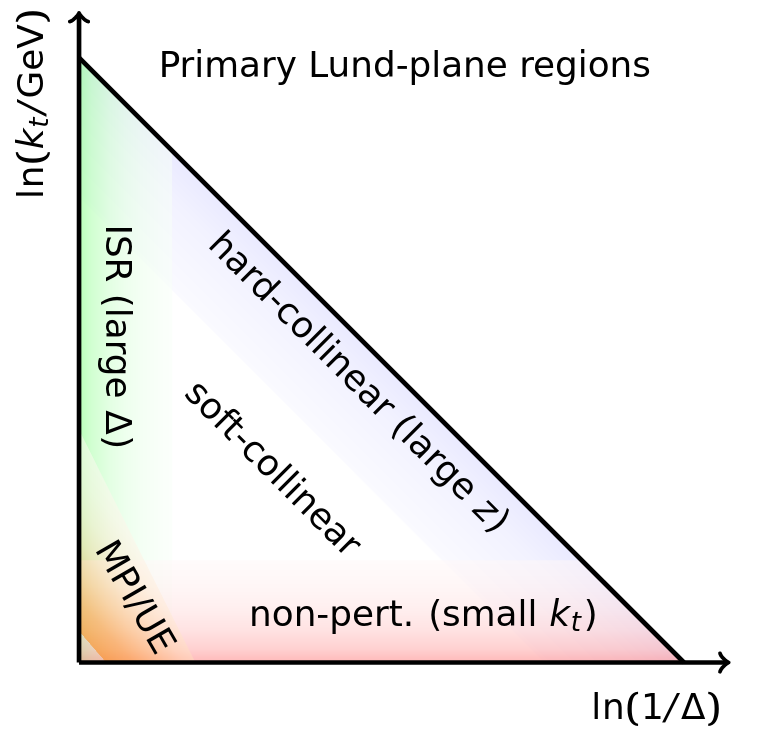
\includegraphics[width=0.45\textwidth]{lund_plane}
\caption{The kinematic regions within the primary Lund Jet Plane \cite{Dreyer:2018nbf}.}
\label{LundPlane}
\end{figure}

For the sake of completeness, we would like to mention that a splitting is characterised not just by the ($\Delta, k_t$) coordinates, but also by
\begin{equation}
\begin{cases}
 z = \frac{p_{Tb}}{p_{Ta}+p_{Tb}} \\
 m^2 = (p_a + p_b)^2 \\
 \psi = \tan^{-1} \frac{y_b - y_a}{\phi_b - \phi_a}.
\end{cases}
\label{z m psi}
\end{equation}
There exist also alternative representations of the Lund Plane, where instead of $\ln(k_t/\mathrm{GeV})$, $\ln(1/z)$ is shown. These other Lund coordinates have been used to train graph neural network based taggers, such as LundNet \cite{Dreyer:2020brq}. 

It is also possible to define Lund Planes beyond the primary, by considering further splittings off of the emitted subjets when present. This leads to the definition of secondary planes, tertiary planes, etc. This process is shown in Figure \ref{emissions}.

\begin{figure}
\centering
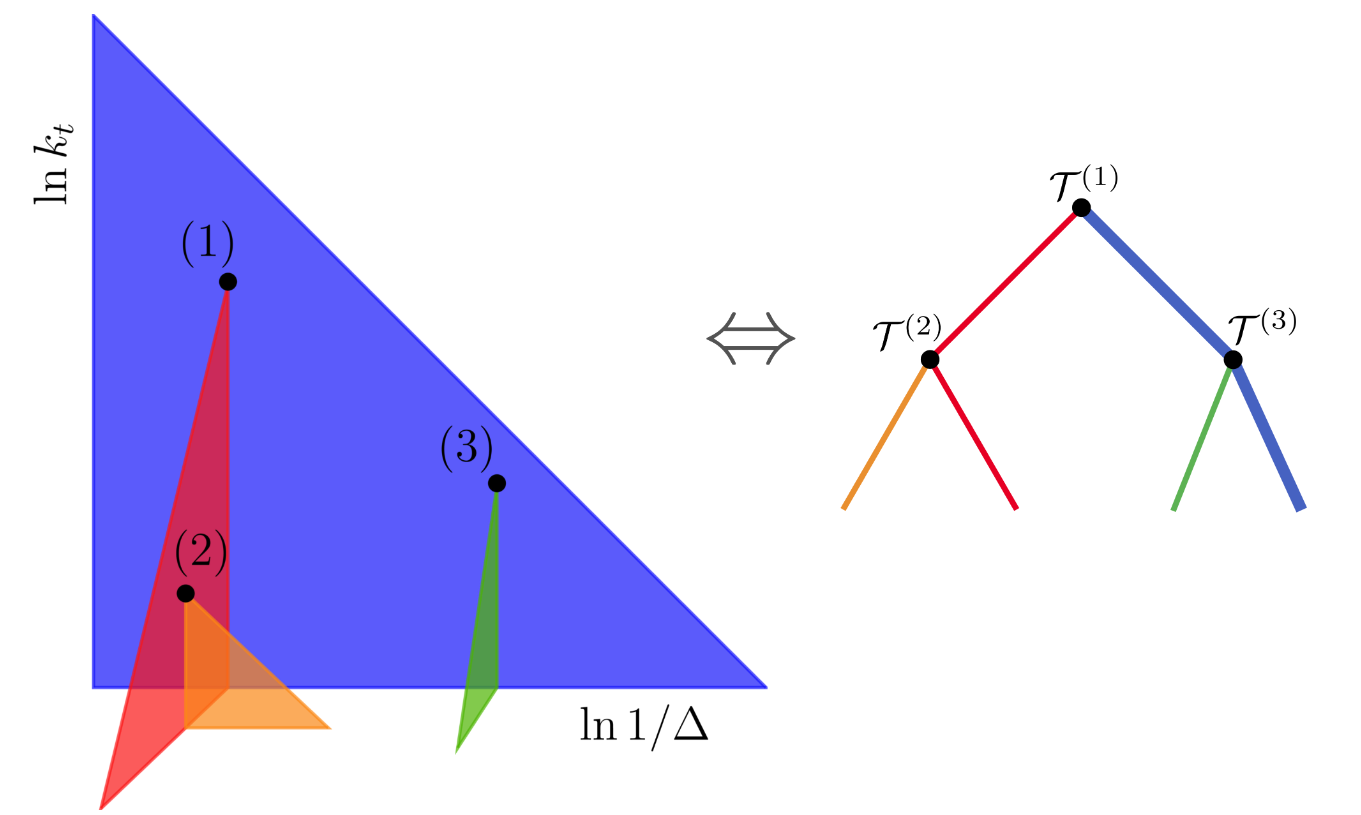
\includegraphics[width=0.7\linewidth]{emissions}
\caption{The primary Lund Plane for a hypothetical jet with emissions (1) and (3), and the secondary Lund Plane (2) from branch (1) and corresponding tree structure of the jet showing this evolution. Each splitting can be charachterised by the set of Lund variables $\mathcal{T}$, given by Eq. \ref{delta kt} and Eq. \ref{z m psi} \cite{Dreyer:2020brq}.}
\label{emissions}
\end{figure}

The Lund Plane has been measured on inclusive jets by the ATLAS, CMS and ALICE collaborations \cite{ATLAS:2020bbn, CMS:2023lpp, ALICE:2021yet}. ATLAS has additionally released measurements for the Lund Plane for top and W jets \cite{ATLAS:2024dua} and a measurement on the Lund subjet multiplicity \cite{ATLAS:2024wrd}.

\todo{Add citations to CMS dead cone papers/LHCb paper}

%parlare del lavoro 

%Discuss what is a parton shower
%How Lund Diagrams are useful
%Discuss Panscales and NLL accurate showers
 
\subsection{Modified jet angularities}

The generalised angularities \cite{Larkoski:2014pca, Proceedings:2018jsb, Gras:2017jty}, henceforth referred to as just \emph{angularities}, are a class of observables designed for quark/gluon jet discrimination. They are defined as 

\begin{equation}
\lambda^\kappa_\alpha = \sum_i \left(\frac{p_{Ti}}{p_{Tjet}}\right)^\kappa \left(\frac{\Delta R_i}{R_0} \right)^\alpha
\end{equation} 
where the sum runs over all constituents of an anti-$k_t$ jet of radius $R_0$, and $\Delta R_i$ indicates the distance between the $i$-th constituent and the jet axis. $\lambda^\kappa_\alpha$ is IR-safe for $\kappa \geq 1$, and we shall assume $\kappa = 1$ going forward, unless otherwise specified.

A few angularities are distinguished enough to have their own name. These include $\lambda_1$, known as the \emph{jet width} and $\lambda_2$, known as the \emph{jet thrust}, amongst others. The idea behind these and other angularities is to emphasise various aspects of a jet's substructure in order to highlight features typical of quark or gluon jets. By tuning the $\beta$ parameter, one can accentuate either wide-angle or collinear radiation, while tuning the $\kappa$ parameter has the same effect on harder or softer hadrons. Ultimately, the difference between quark and gluon jets originates from the fact that $C_A > C_F$, implying that gluons are more likely to emit soft and collinear gluons than quarks.

The phenomenology of such observables has been extensively studied at colliders for processes such as $Z$+jets \cite{Reichelt:2021svh} at the LHC, and they have been measured in proton-proton collisions by the ATLAS, CMS and ALICE collaborations on a variety of energies and final states \cite{ATLAS:2019kwg, CMS:2021vsp, ALICE:2021njq, Dhankher:2024rkv}.

Recently, a proposal for modified angularities has been put forth \cite{Dhani:2024gtx}. 

The variants are defined by reclustering a jet with the C/A algorithm using the winner-takes-all (WTA) scheme. Two vectors are defined:
\begin{gather}
n_0 = \left(\cosh y, \cos \phi, \sin \phi, \sinh y \right) \\
n = \left(\frac{m_{T, n}}{p_{T, n}} \cosh y, \cos \phi, \sin \phi, \frac{m_{T, n}}{p_{T, n}}\sinh y \right)
\end{gather}

where $\phi$ and $y$ are the azimuthal angle and rapidity of the WTA axis, and $m_{T, n} = p_{T, n} + m_{n}$ is the transverse mass of the particle aligned with the WTA axis. The $(E, p_x, p_y, p_z)$ convention is used to define the vectors.

The variants are then defined as

\begin{align}
\label{lambdaDot}
\dot{\lambda}_0^\alpha &= \sum_i \frac{p_{T,i}}{p_T}\left(\frac{2p_i\cdot n_0}{p_{T,i}R^2} \right)^{\frac{\alpha}{2}}  & 
\dot{\lambda}^\alpha &= \sum_i \frac{p_{T,i}}{p_T}\left(\frac{2p_i\cdot n}{p_{T,i}R^2} \right)^{\frac{\alpha}{2}} \\
\label{lambdaHat}
\hat{\lambda}_0^\alpha &= \sum_{i\neq n} \frac{p_{T,i}}{p_T}\left(\frac{2p_i\cdot n_0}{p_{T,i}R^2} \right)^{\frac{\alpha}{2}}  &
\hat{\lambda}^\alpha &= \sum_{i\neq n} \frac{p_{T,i}}{p_T}\left(\frac{2p_i\cdot n}{p_{T,i}R^2} \right)^{\frac{\alpha}{2}}.
\end{align}

where the sums in Eqs.~\ref{lambdaHat} excludes the particle aligned with the WTA axis. 
These variants are specifically designed to bring to light the mass of the particle aligned with the WTA-axis. Considering jets seeded by heavy flavour partons and suppress the decay of the corresponding hadrons, the particle aligned with the WTA axis will be a hadron containing the same flavour of quark which seeded the jet. As such, the observables defined in Eq.~\ref{lambdaDot} will contain an \emph{explicit mass dependence}. In the quasi-collinear limit, for example,

\begin{equation}
\dot{\lambda}^\alpha_0 \approx \sum_{i \neq n}\frac{p_{T,i}}{p_T}\left(\frac{m_i^2}{p_{T,i}^2R^2} + \frac{\Delta R_i^2}{R^2} \right)^{\frac{\alpha}{2}} + \left(\frac{m_n^2}{p_{T,n}^2R^2} \right)^{\frac{\alpha}{2}}.
\end{equation}

The end result is a set of observables (Eq.~\ref{lambdaHat}) sensitive to quark mass. 

\textcolor{red}{Show plots from paper??}

\subsection{Other variables of interest}
\textcolor{red}{Colour ring, D2,boosted kinematic variables, etc.}

\section{Object selections and event definitions}

\subsection{Data Pre-selection}

This analysis makes use of data recorded with the ATLAS experiment during Run 2, corresponding to the years 2015-2018. The events consist of $pp$ collisions at $\sqrt{s} = $13~TeV during stable beam conditions with all subsystems of the detector operational and passing all data quality requirements. Overall, the data amounts to $139$~fb$^{-1}$. 

\subsection{Definition of signal regions}

As mentioned, the analysis aims to understand the substructure of b-jets and does so by making comparisons to light jets. To this aim, the signal corresponds to $Z$-boson production in association with two jets, either both b-tagged or both anti-b-tagged. Leptonic decays of the $Z$-boson are considered, either to an $e^+e^-$ or $\mu^+\mu^-$ pair. 

Two topologies are considered: a resolved topology where the jets are sufficiently separated to be identified as two separate anti-$k_t$ jets of radius $R = 0.4$. In this case, PFlow jets are considered and the substructure observables are measured on these jets. A boosted topology is also considered, where, in this case, the jets are produced at high $p_T$ and as a result are too close together to be fully resolved. In this case, two VR-trackjets, both b- or anti-b- tagged, are required to lie within a large-R LCTopoJets of radius $R = 1.0$, which is taken to be the signal jet for the measurement. Overall, we are left with four signal regions: resolved 2B, resolved 0B, boosted 2B, and boosted 0B.


\subsection{Lepton selections}
Electron candidates are identified from energy clusters in the electromagnetic calorimeter that are linked to reconstructed tracks in the Inner Detector. Candidates must be found within the calorimeter, i.e. within $\vert \eta \vert < 2.47$, excluding the transition region between 1.37 < $\vert \eta \vert$ 1.52. In order to qualify as electrons, they must meet the TightLH identification criterion and satisfy additional requirements on their transverse and longitudinal impact parameters: $\vert z_0\sin(\theta)\vert  < 0.5$~mm and $\vert d_0/\sigma(d_0)\vert < 5.0$. To further minimize background from non-prompt electrons, conversions, and hadrons, candidates are required to be meet isolation criteria and must pass the Tight\_VarRad isolation working point. This equates to having both the calorimeter energy sum and $p_T$ sum of the tracks within a variable radius cone (up to a maximum radius of $\Delta R = 0.2$) centred around the electron less than $0.06 E_T$, where $E_T$ indicates the transverse energy. Lastly, electrons must meet specific criteria regarding the shape of the electromagnetic shower, track quality, and track alignment with respect to the calorimeter cluster. A likelihood based method with a ``Tight" working point is utilised to satisfy these selections.

Muon candidates are identified by correlating tracks found within the inner detector to tracks or track segments in the muon spectrometer. They must meet impact parameter criteria of $\vert z_0\sin(\theta)\vert  < 0.5$~mm and $\vert d_0/\sigma(d_0)\vert < 3.0$ and pass the "Medium" identification working point, based on quality requirements on the tracks in the inner detector and the muon spectrometer. In addition, muons must pass the``FCTight FixedRad” working point to pass isolation requirements. The $p_T$ sum of tracks in a variable radius cone (maximum radius $\Delta R = 0.3$) centred around the muon must be no more than $0.04$ times the muon $p_T$. Lastly, muons must be found at pseudorapidities $\vert \eta \vert < 2.5$. 

Both electrons and muons must have a $p_T < 27$~GeV.

\subsection{Jet selections}

\subsubsection{Resolved SRs}
In the resolved signal regions, jets are clustered using the anti-$k_t$ algorithm as implemented in the FastJet package with PFlow objects are constituents. PFlow objects are constructed by matching tracks to calorimeter clusters, and subtracting the contribution of the energy deposit in the calorimeter due to the particles from which the tracks originate. 

The algorithm works as follows: a set of ``well-measured'' tracks with  a track fit of $\chi^2/dof < 5$, where ``dof'' stands for ``degrees of freedom'' is identified. Tracks are matched to a single topocluster in the calorimeter. For each track/topocluster pair, the probability that the particle giving origin to the track deposits its energy in more than topocluster is determined, and, if this is found to be the case, additional topoclusters are added to the system considered so as to reconstruct the full shower. A cell-by-cell subtraction of the energy of the particle then occurs, and a list of tracks, topoclusters, and charged-particle energy-subtracted topoclusters is then returned. 

The PFlow objects are matched to the primary vertex, and clustered using the anti-$k_t$ algorithm, as stated above. The radius parameters chosen are either $R = 0.4$ for small-R jets, or $R = 1.0$ for large-R jets. Calibrations which correct for the effects due to reconstruction, such as the presence of pile-up, are then applied. These include the jet-energy scale (JES) and jet-energy resolution (JER) calibrations.

Jets in these signal regions must satisfy $p_T > 20$~GeV and $\vert y \vert < 2.5$. The jet vertex tagger (JVT) discriminant is used to reject jets originating from pileup vertices, with a ``Tight" working point, corresponding to a JVT value above 0.5 for jets in the $p_T$ range $20 \, \text{GeV} < p_T < 60 \, \text{GeV}$ and with pseudorapidity $\vert \eta \vert < 2.4$. \todo{Do we really care about the specific JVT value? The WP should be enough.}

Jets in the resolved signal regions are (anti) b-tagged using the DL1r  b-tagging discriminant. Jets are considered (anti) b-tagged if they (fail) pass the 70\% efficiency working point, corresponding to 70\% efficiency in identifying jets containing b-hadrons. This working point is also characterised by a c-jet rejection rate of 10, and a light jet rejection rate of 417, indicating that 1/10 or 1/417 jets will be mistagged, respectively. 

\subsubsection{Boosted SRs}

Two jet collections are utilised in the boosted regimes. Large-R jets of radius $R = 1.0$, clustered with the anti-$k_t$ algorithm from the FastJet package. These jets are clustered with locally-calibrated topological (LCTopo) clusters of energy from the hadronic calorimeter.  This method aims to calibrate the calorimeter signals on a cluster-by-cluster basis to account for signal losses due to the clustering of the calorimeter cells, compensate for energy loss in inactive materials, and account for the limitations of a non-compensating calorimeter. In order to generate the input 4-vectors for the clustering algorithm, the topoclusters are directed to align with the primary vertex.

The large-R jets are also trimmed. Trimming is a type of grooming which reclusters a jet's constituents into subjets with a radius $R_{sub}$ and removes any constituents associated with a subjet carrying a fraction of $p_T$ less than $f_\mathrm{cut}$. The $k_t$ algorithm is chosen specifically as it clusters soft particles first. In this case, the trimming parameters correspond to $R_{\mathrm{sub}} = 0.2$ and $f_{\mathrm{cut}} = 0.05$. 

Large-R jets are tagged through the use of variable radius (VR) trackjets matched to the jet of interest. These jets, composed of tracks only, are characterised, as their name may imply, by a radius parameter which varies with the $p_T$ of the jet. The radius parameter varies as follows:
\begin{equation}
R \rightarrow R_{eff}{p_{T,i}} = \frac{\rho}{p_{T,i}}
\label{Reff}
\end{equation} 

where $R_{eff}$ is an effective radius parameter dependent on the transverse momentum of the proto-jet $p_{T,i}$. $\rho$ is a parameter which determines the speed with which the effective radius decreases. It is set to $\rho = 30$ GeV. The jet radius varies according to \ref{Reff}, up to (down to) a maximum (minimum) radius of $R = 0.4$ ($R = 0.02$). Overall, the radius paramter is given by 
\begin{equation}
R = max(0.02, min(0.4, \frac{\rho}{p_T}).
\end{equation}



\subsection{Track selections}
\label{track sel}
Tracks are reconstructed from hits of charged particles detected in the inner tracker. They must meet the ``Loose'' quality working point. This corresponds to a satisfying a $p_T > 500 MeV$ cut and $\vert \eta \vert < 2.5$ cut, as well as requiring at least eight hits in the silicon layers (pixel and SCT), no more than one shared module between the pixel detector and SCT, no more than one hole in the pixel detector and no more than two holes total in the pixel layers. For the sake of this measurement, the track $p_T$ requirement was increased to 900 MeV.

Tracks must also satisfy the ``Loose'' working point of the TrackVertexAssociation tool to ensure that they are matched to the primary vertex. This selection corresponds to requiring that the track was used in any track fit, and that the $\vert z_0 \sin\theta \vert < 3$ mm.

The working points and $p_T$ threshold were optimised to ensure the highest number of matches between emissions at truth and reco level for IBU unfolding (add plot). It is important to note that this does not necessarily ensure that the number of fakes and inefficiencies is minimised, just that, per happenstance, the number of fakes and inefficiencies is such that the total number of emissions in the primary lund plane matches between truth and reco level.

\subsection{Primary vertex}

In each event, it is important to properly reconstruct the primary vertex of the proton-proton scattering in order to define a reference point from which to calculate track and vertex displacements. The primary vertex is identified as the point with the highest $p_T^2$ sum of contributing tracks. Each event analysed is required to have at least one primary vertex.

\subsection{Event selection}

\section{Lund plane (and angularities) reconstruction}

The Lund Plane is reconstructed from tracks satisfying the requirements described in \ref{track sel}. The measurement does not include calorimeter cells due to the better angular resolution of the Inner Tracker. 

\todo{add plot comparing to pflow and ufo}

Tracks and/or the reconstructed B-hadron are matched to jets through a geometric matching, by which a track is required to be within a distance $\Delta R$ from the jet axis equal to the jet radius. The tracks matched to each jet are then clustered into a jet using the anti-$k_t$ algorithm, and the Lund Plane algorithm is subsequently applied as described in \ref{lp sec}.

The working points and $p_T$ threshold used in the track selection were optimised to ensure the highest number of matches between emissions at truth and reco level for IBU unfolding \todo{(add plot)}. It is important to note that this does not necessarily ensure that the number of fakes and inefficiencies is minimised, just that, per happenstance, the number of fakes and inefficiencies is such that the total number of emissions in the primary lund plane matches between truth and reco level.


The effect of omitting the neutral component was studied at truth level. In figure ...

\section{bkg characterisation/ttbar rejection}

\section{B hadron reconstruction}
To be able to accurately study the substructure of heavy flavour jets, one must solve the problem of the heavy flavour hadron decay products. 

A quark in the final state will radiate gluons, with each subsequent gluon being emitted at a smaller angle in accordance with the DGLAP equations. The radiation may, in turn, emit more radiation, leading to the tree-like structure we call a jet. This structure is mostly preserved after hadronisation.

Heavy flavour hadrons, however, will decay into light hadrons via the weak interaction. To a jet clustering algorithm, the decay products will rightly appear as just another emission as there is no way to distinguish one from the other in data. To get around this issue, theorists will often publish predictions for processes at either parton level or artificially inhibit the decay of the heavy flavour hadron if at hadron level. 

In this measurement, we opt to reconstruct the heavy flavour hadron from it's charged decay products, similar to the strategy adopted by the CMS collaboration in \cite{CMS:2024gds}. Here, the charged momentum of the heavy flavour hadron is reconstructed via tracks identified as coming from the decay by a Boosted Decision Tree trained for this task. We, on the other hand, adopt a cut-based approach. 

The B-hadron is reconstructed through a cut on the track signed impact parameter significance, or $d_0/\sigma(d_0)$. The impact parameter is a measure of the displacement of the track in three-dimensional space from the primary vertex. As such, tracks originating from secondary vertices are characterised by large values of $d_0$ in magnitude. By dividing by the uncertainty on the value of $d_0$, even larger values are assigned to tracks whose $d_0$ is precisely known, further increasing the value for those tracks originating from points other than the primary vertex. The sign comes from the position in three-dimensional space of the track with respect to the axis of the jet which contains it; if the track is in front of the jet axis, a positive value is assigned, whereas if it is behind a negative value is assigned, as shown in Figure \ref{d0sig}. This signed $d_0$ significance makes up the IP3D algorithm, used as one of the inputs for the DL1r flavor tagging algorithm \cite{ATLAS:2022qxm}.

\begin{figure}
    \centering
    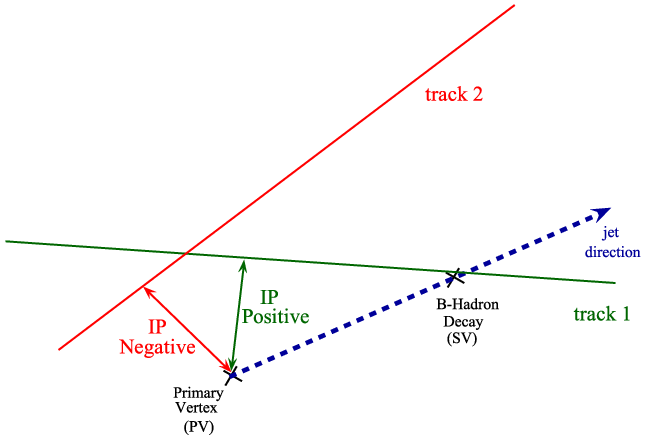
\includegraphics[width=0.7\linewidth]{signedD0}
    \caption{An illustration showing the definition of impact parameter and the associated sign convention.}
    \label{d0sig}
\end{figure}

In Fig. \ref{pflowD0} the signed $d_0$ significance distribution for tracks associated to PFlow jets tagged as b-jets or light jets is shown. From here, it is clear that the observable chosen has discrimination potential.

\begin{figure}
    \centering
    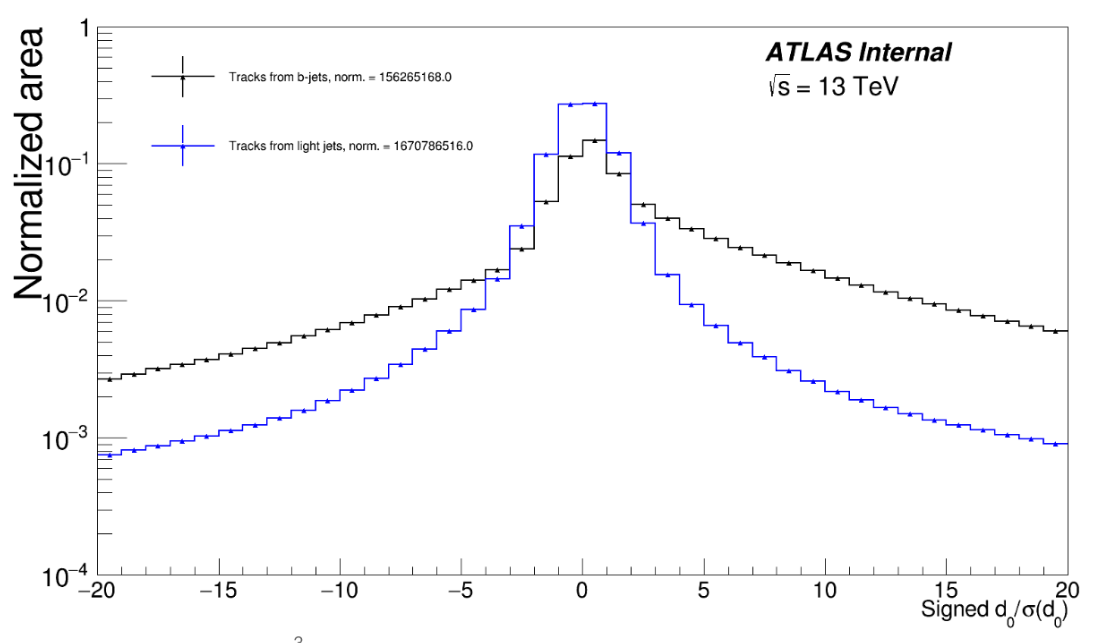
\includegraphics[width=\linewidth]{pflowD0}
    \caption{The distribution of the signed $d_0$ significance for tracks in PFlow jets tagged as b-jets (black) vs. the same distribtuion for tracks associated in PFlow jets tagged as light jets (blue).}
    \label{pflowD0}
\end{figure}

To reconstruct the B hadron from its charged decay products, a detailed study was undertaken to optimise the track selection. The reconstruct B hadron four-momentum, namely $p_T$, $y$ and $\phi$ was optimised against the truth B-hadron partially reconstructed from only its charged decay products. 

It was found that tracks satisifying the requirement $d_0/\sigma(d_0) > 0.5$ or signed $d_0/\sigma(d_0) < -4$ best reproduced the truth-level charged four-momentum of the B-hadron. In cases in which no track in a b-jet is found to satisfy these requirements, the leading track is assumed to originate from the decay, in accordance with the leading particle effect. In this way, no additional requirement beyond b-tagging is placed on the jets whose substructure we analyse. Figure \ref{chargedMigration} shows the migration of the charged B hadron momentum from truth level to reco level using tracks satisfying these selections.

\begin{figure}
    \centering
    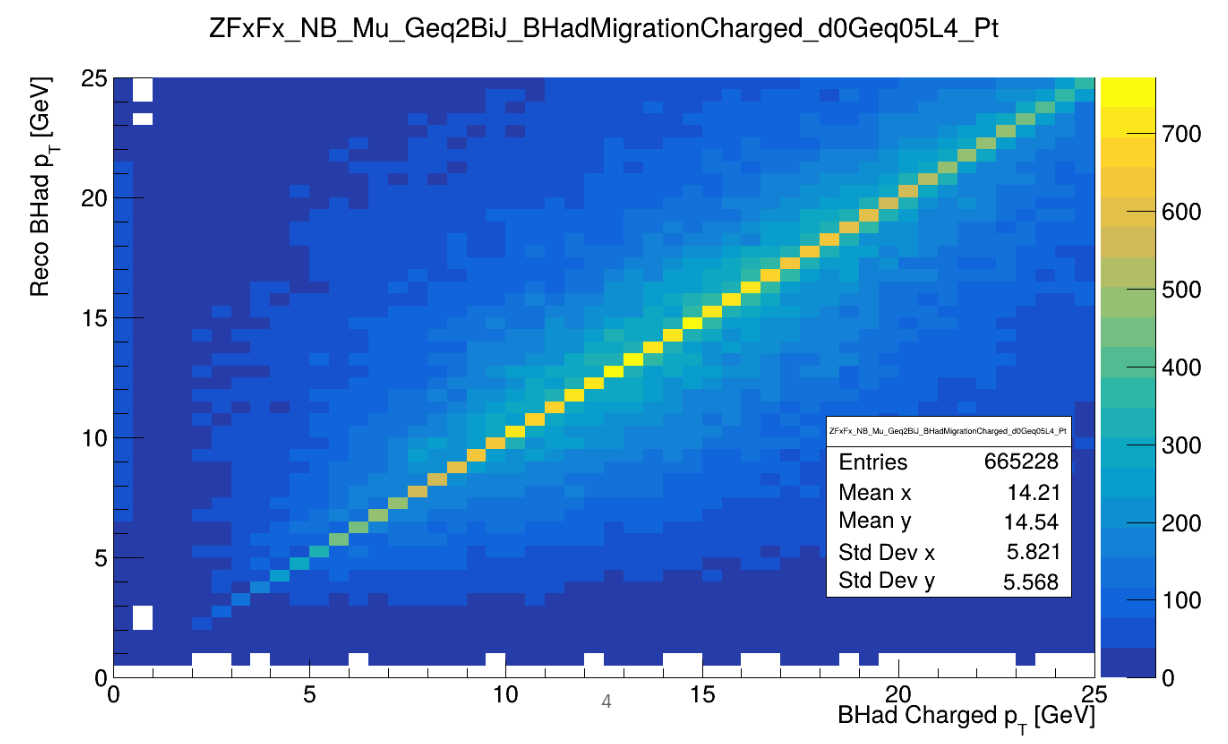
\includegraphics[width=0.9\linewidth]{analysis-chapter/pflowMig_pt.png}
    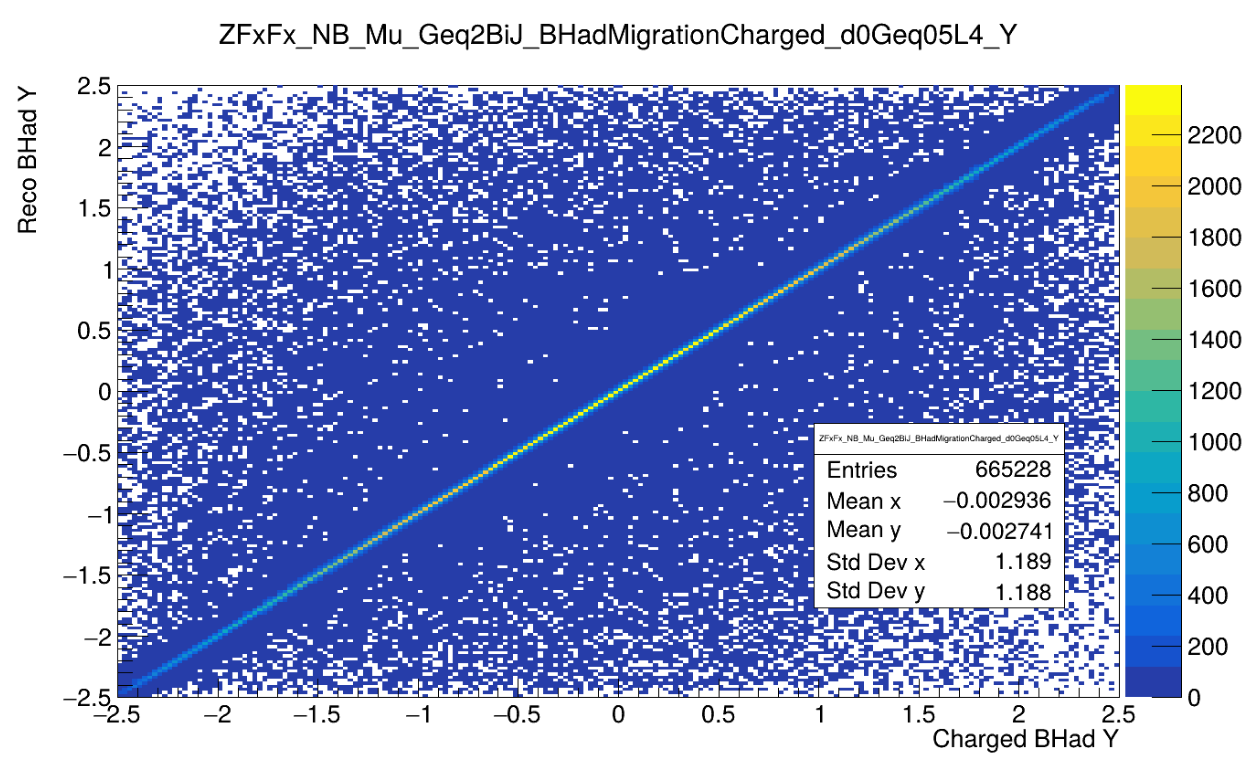
\includegraphics[width=0.9\linewidth]{analysis-chapter/pflowMig_y.png}
    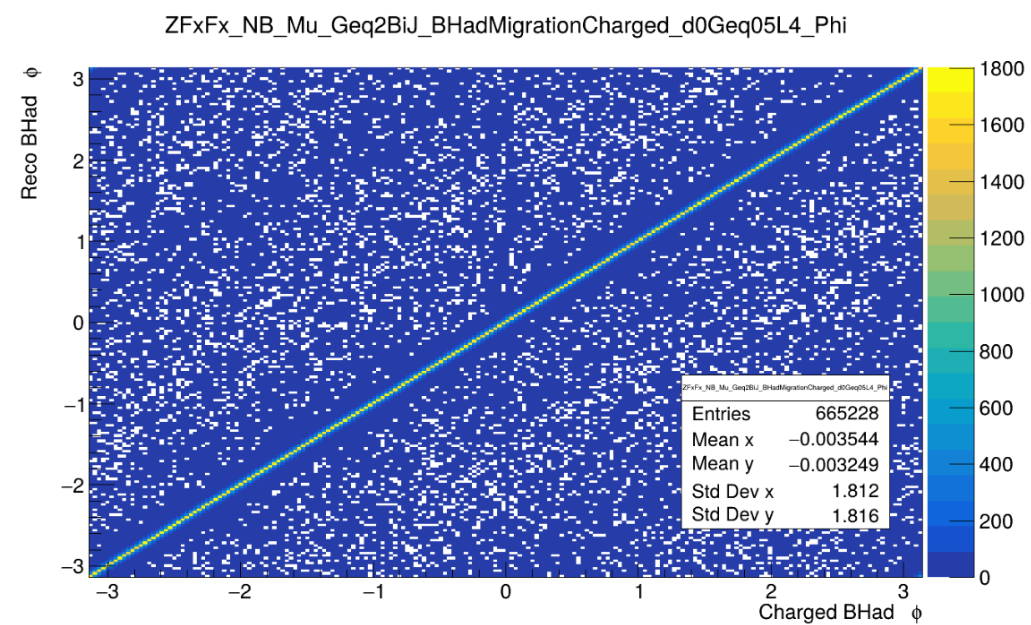
\includegraphics[width=0.9\linewidth]{analysis-chapter/pflowMig_phi.png}
    \caption{The reconstructed B Hadron $p_T$, $y$, and $phi$ vs. that obtained via the sum of the charged decay products of the B hadron at truth level.}
    \label{chargedMigration}
\end{figure}


Figure \todo{blah}, on the other hand, shows the migration of the reconstructed B Hadron four-momentum when compared against the full, undecayed truth B Hadron, rather than just the component obtained from the charged decay products. From here, it is clear that, although the $p_T$ of the reconstructed B Hadron tends to underestimate that of the undecayed truth B Hadron, the $y$ and $\phi$ distributions do not change much.

\begin{figure}
    \centering
    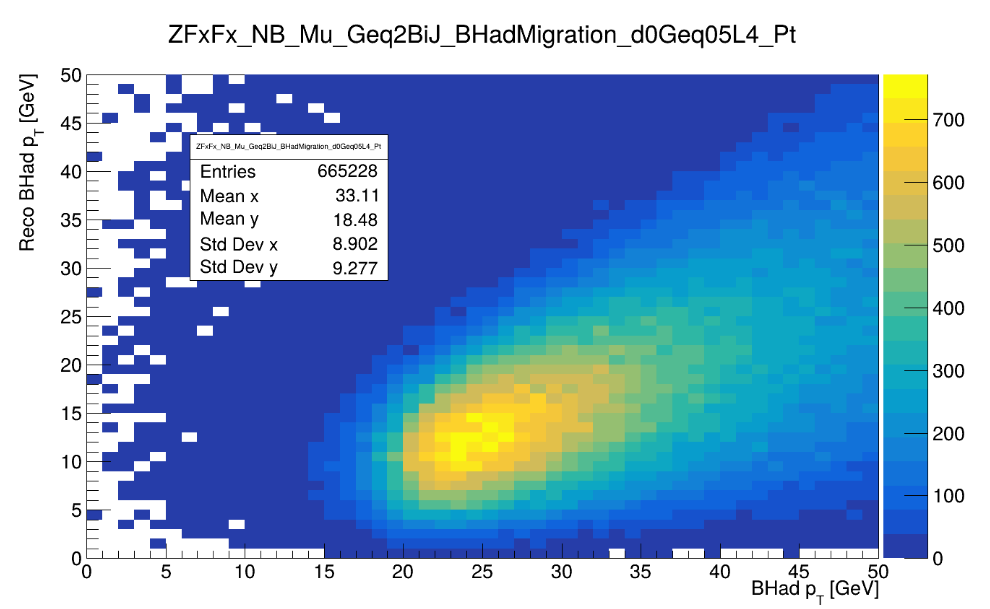
\includegraphics[width=0.9\linewidth]{analysis-chapter/pflowMig_tot_pt.png}
    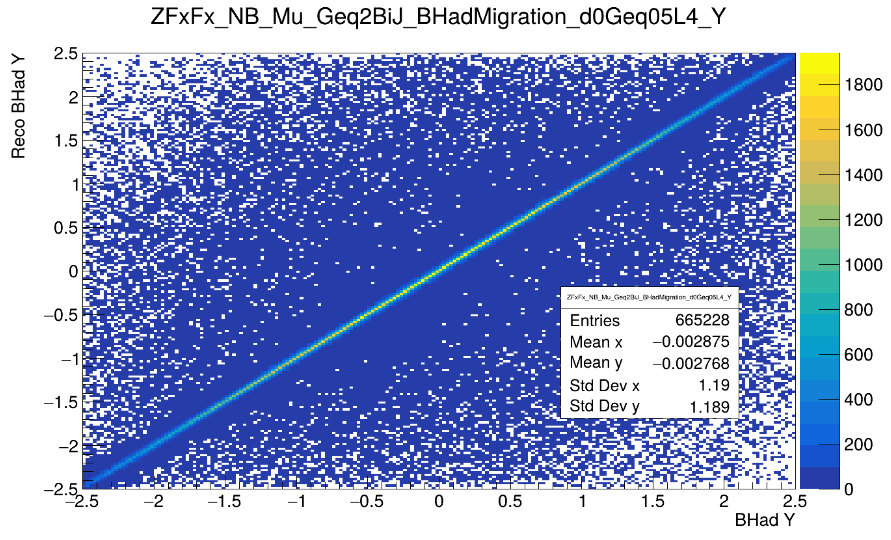
\includegraphics[width=0.9\linewidth]{analysis-chapter/pflowMig_tot_y.png}
    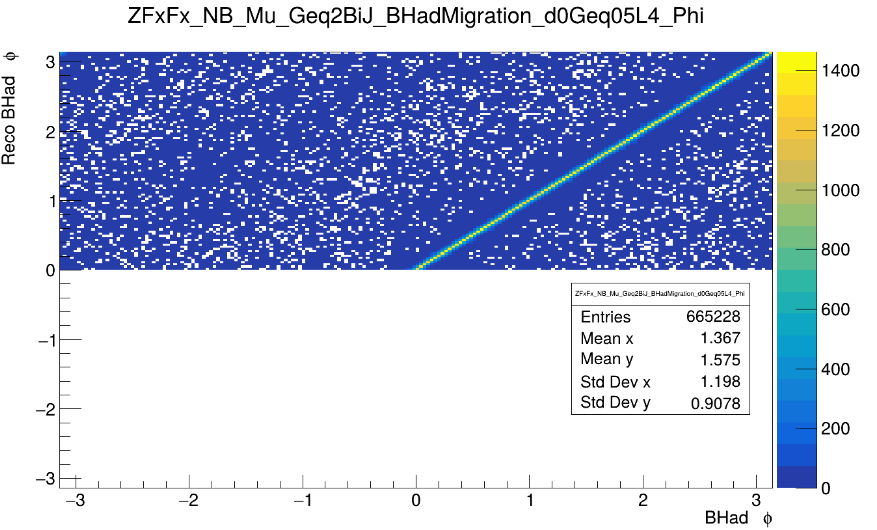
\includegraphics[width=0.9\linewidth]{analysis-chapter/pflowMig_tot_phi.png}
    \caption{The reconstructed B Hadron $p_T$, $y$, and $phi$ vs. that of the undecayed truth-level B Hadron.}
    \label{chargedMigration}
\end{figure}

Up to now, the discussion of B Hadron reconstruction has been focused on tracks associated to PFlow jets. Although there is no reason to expect why this should not hold true for tracks associated to boosted jets, the effectiveness of the reconstruction was also checked in this case.

In the boosted case, the signed $d_0$ significance distribution for tracks associated to VR trackjets tagged as $b$-jets is studied. Figure \ref{d0Boost} shows the distribution of this variable for tracks in the boosted case vs. the same distribution in the resolved case. No significant difference is observed. For this reason, the same track selections were implemented in the boosted case, and the migration plots are shown in Figure \ref{boostedMigration}. 

\begin{figure}
    \centering
    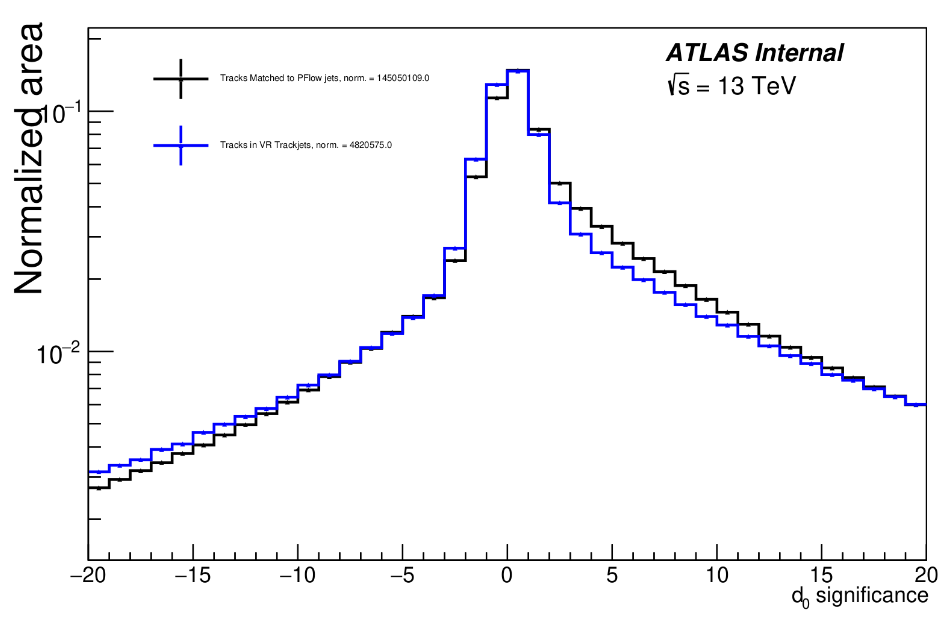
\includegraphics[width=0.9\linewidth]{analysis-chapter/d0Boosted.png}
    \caption{The distribution of the signed $d_0$ significance of tracks in b-jets in the resolved case (black) vs. the boosted case (blue).}
    \label{d0Boost}
\end{figure}

\begin{figure}
    \centering
    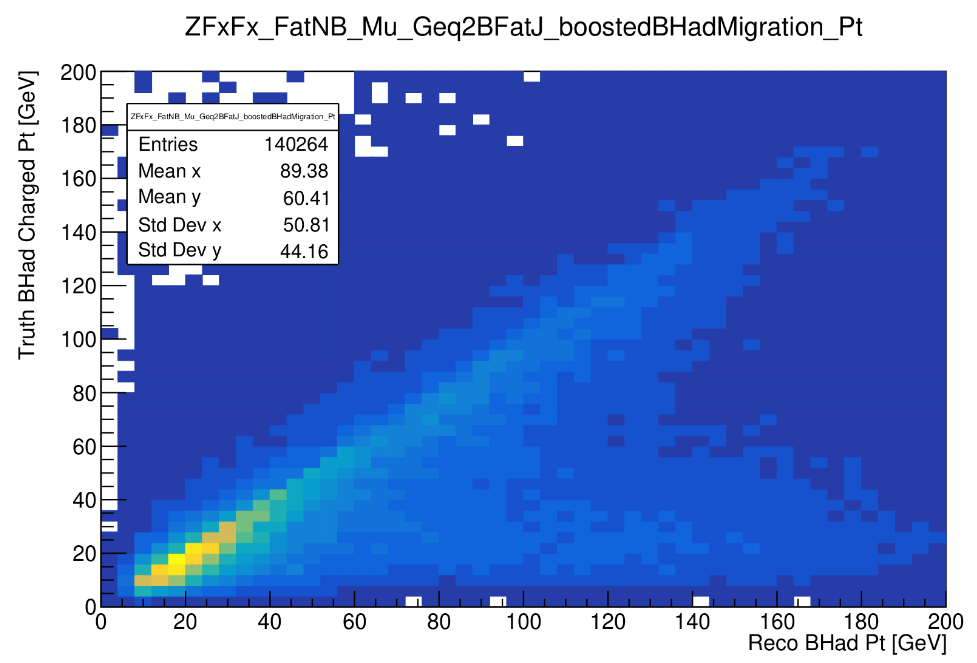
\includegraphics[width=0.9\linewidth]{analysis-chapter/bhadMig_boost_pt.png}
    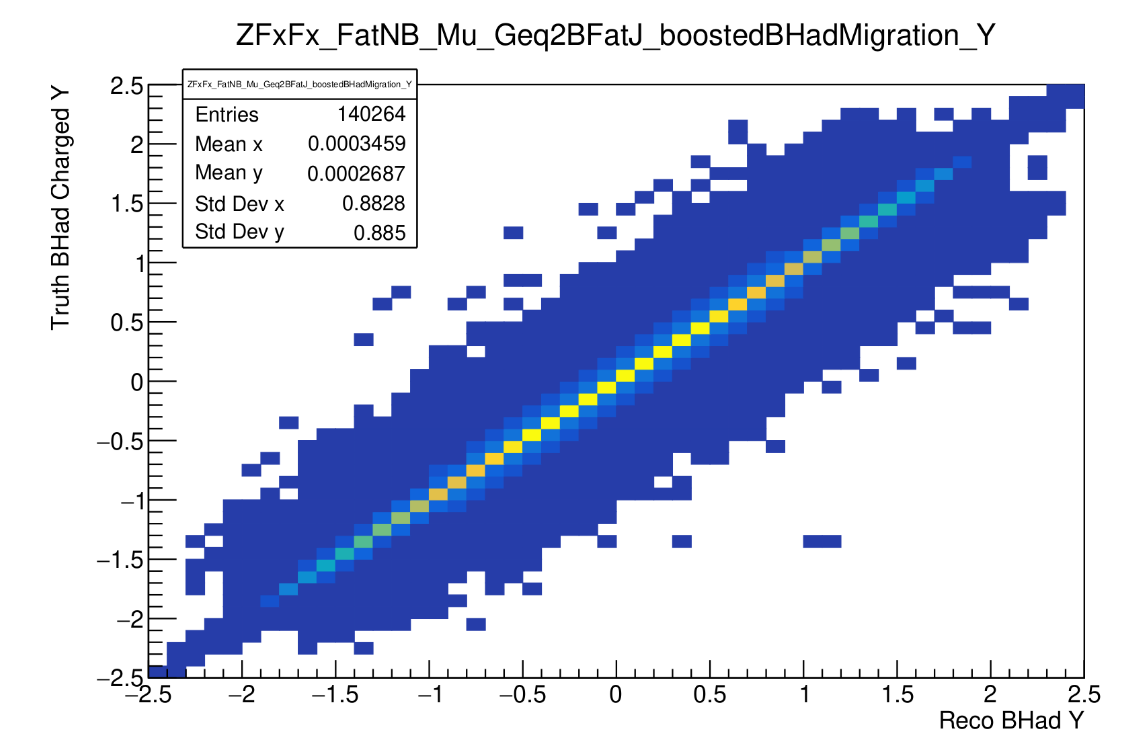
\includegraphics[width=0.9\linewidth]{analysis-chapter/bhadMig_boost_y.png}
    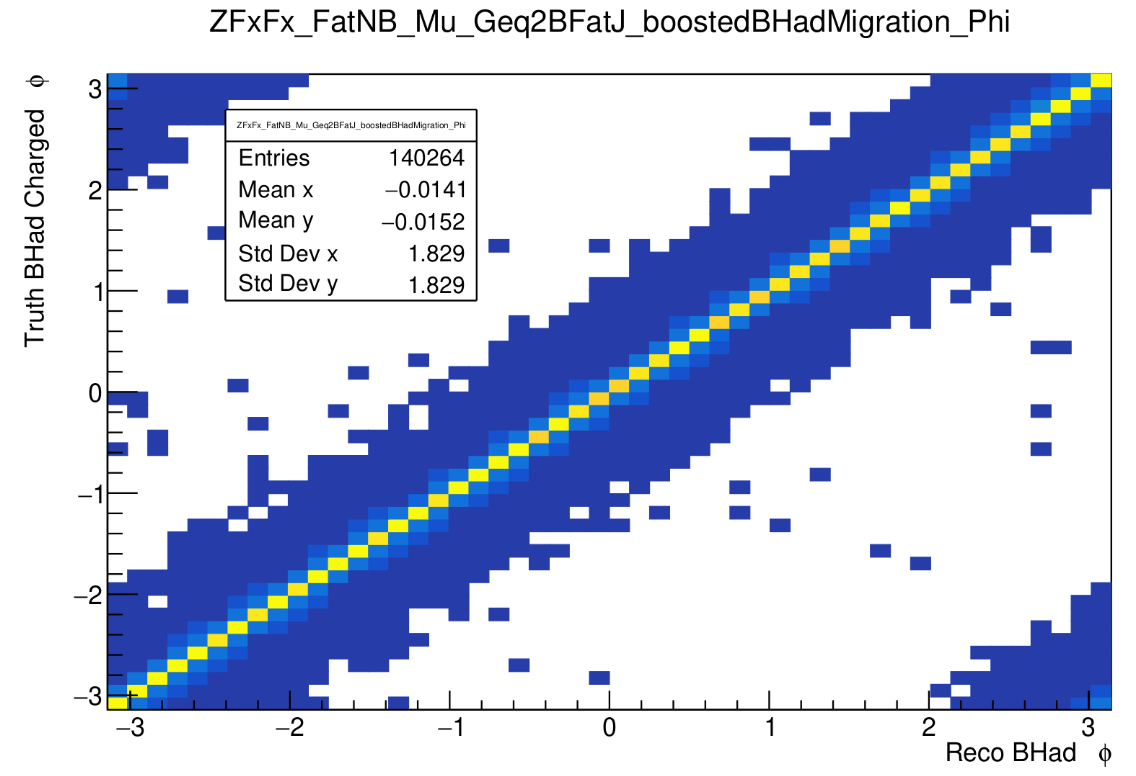
\includegraphics[width=0.9\linewidth]{analysis-chapter/bhadMig_boost_phi.png}
    \caption{The reconstructed B Hadron $p_T$, $y$, and $phi$ vs. that of the truth-level B Hadron reconstructed from its charged decay products in VR trackjets.}
    \label{boostedMigration}
\end{figure}



\end{document}